    \hypertarget{muxe9thodes-spuxe9ciales-33}{%
\section{Méthodes spéciales (3/3)}\label{muxe9thodes-spuxe9ciales-33}}

    \hypertarget{compluxe9ment---niveau-avancuxe9}{%
\subsection{Complément - niveau
avancé}\label{compluxe9ment---niveau-avancuxe9}}

    Ce complément termine la série sur les méthodes spéciales.

    \hypertarget{getattr__-et-apparentuxe9s}{%
\subsubsection{\texorpdfstring{\texttt{\_\_getattr\_\_} et
apparentés}{\_\_getattr\_\_ et apparentés}}\label{getattr__-et-apparentuxe9s}}

    Dans cette dernière partie nous allons voir comment avec la méthode
\texttt{\_\_getattr\_\_}, on peut redéfinir la façon que le langage a
d'évaluer~:

\begin{verbatim}
objet.attribut
\end{verbatim}

    \textbf{Avertissement~:} on a vu dans la séquence consacrée à l'héritage
que, pour l'essentiel, le mécanisme d'héritage repose
\textbf{précisément} sur la façon d'évaluer les attributs d'un objet,
aussi nous vous recommandons d'utiliser ce trait avec précaution, car il
vous donne la possibilité de ``faire muter le langage'' comme on dit.\\

    \textbf{Remarque~:} on verra en toute dernière semaine que
\texttt{\_\_getattr\_\_} est \emph{une} façon d'agir sur la façon dont
le langage opère les accès aux attributs. Sachez qu'en réalité, le
protocole d'accès aux attributs peut être modifié beaucoup plus
profondément si nécessaire.

    \hypertarget{un-exemple-la-classe-rpcproxy}{%
\subparagraph{\texorpdfstring{Un exemple~: la classe
\texttt{RPCProxy}}{Un exemple~: la classe RPCProxy}\\\\}\label{un-exemple-la-classe-rpcproxy}}

    Pour illustrer \texttt{\_\_getattr\_\_}, nous allons considérer le
problème suivant. Une application utilise un service distant, avec
laquelle elle interagit au travers d'une API.\\

C'est une situation très fréquente~: lorsqu'on utilise un service météo,
ou de géolocalisation, ou de réservation, le prestataire vous propose
une \textbf{API} (Application Programming Interface) qui se présente
bien souvent comme une \textbf{liste de fonctions}, que votre fonction
peut appeler à distance au travers d'un mécanisme de \textbf{RPC}
(Remote Procedure Call).\\

Imaginez pour fixer les idées que vous utilisez un service de
réservation de ressources dans un Cloud, qui vous permet d'appeler les
fonctions suivantes~:

\begin{itemize}
\tightlist
\item
  \texttt{GetNodes}(\ldots{}) pour obtenir des informations sur les
  noeuds disponibles~;
\item
  \texttt{BookNode}(\ldots{}) pour réserver un noeud~;
\item
  \texttt{ReleaseNode}(\ldots{}) pour abandonner un noeud.
\end{itemize}

    Naturellement ceci est une API extrêmement simplifiée. Le point que nous
voulons illustrer ici est que le dialogue avec le service distant~:

\begin{itemize}
\tightlist
\item
  requiert ses propres données - comme l'URL où on peut joindre le
  service, et les identifiants à utiliser pour s'authentifier~;
\item
  et possède sa propre logique - dans le cas d'une authentification par
  session par exemple, il faut s'authentifier une première fois avec un
  login/password, pour obtenir une session qu'on peut utiliser dans les
  appels suivants.
\end{itemize}

    Pour ces raisons il est naturel de concevoir une classe
\texttt{RPCProxy} dans laquelle on va rassembler à la fois ces données
et cette logique, pour soulager toute l'application de ces détails,
comme on l'a illustré ci-dessous~:\\

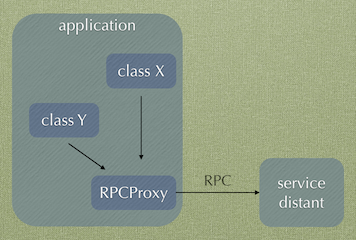
\includegraphics{medias/rpcproxy.png}\\

    Pour implémenter la plomberie liée à RPC, à l'encodage et décodage des
données, et qui sera interne à la classe \texttt{RPCProxy}, on pourra en
vraie grandeur utiliser des outils comme~:

\begin{itemize}
\tightlist
\item
  \href{https://docs.python.org/3/library/xmlrpc.client.html}{\texttt{xmlrpc.client}}
  qui fait partie de la bibliothèque standard~;
\item
  ou, pour JSON, une des nombreuses implémentations qu'un moteur de
  recherche vous exposera si vous cherchez \texttt{python\ rpc\ json},
  comme par exemple
  \href{https://pypi.python.org/pypi/json-rpc/}{\texttt{json-rpc}}.
\end{itemize}

Cela n'est toutefois pas notre sujet ici, et nous nous contenterons,
dans notre code simplifié, d'imprimer un message.

    \hypertarget{une-approche-nauxefve}{%
\subparagraph{Une approche naïve\\\\}\label{une-approche-nauxefve}}

    Se pose donc la question de savoir quelle interface la classe
\texttt{RPCProxy} doit offrir au reste du monde. Dans une première
version naïve on pourrait écrire quelque chose comme~:

    \begin{Verbatim}[commandchars=\\\{\}]
{\color{incolor}In [{\color{incolor}1}]:} \PY{c+c1}{\PYZsh{} la version naïve de la classe RPCProxy}
        
        \PY{k}{class} \PY{n+nc}{RPCProxy}\PY{p}{:}
            
            \PY{k}{def} \PY{n+nf}{\PYZus{}\PYZus{}init\PYZus{}\PYZus{}}\PY{p}{(}\PY{n+nb+bp}{self}\PY{p}{,} \PY{n}{url}\PY{p}{,} \PY{n}{login}\PY{p}{,} \PY{n}{password}\PY{p}{)}\PY{p}{:}
                \PY{n+nb+bp}{self}\PY{o}{.}\PY{n}{url} \PY{o}{=} \PY{n}{url}
                \PY{n+nb+bp}{self}\PY{o}{.}\PY{n}{login} \PY{o}{=} \PY{n}{login}
                \PY{n+nb+bp}{self}\PY{o}{.}\PY{n}{password} \PY{o}{=} \PY{n}{password}
                
            \PY{k}{def} \PY{n+nf}{\PYZus{}forward\PYZus{}call}\PY{p}{(}\PY{n+nb+bp}{self}\PY{p}{,} \PY{n}{functionname}\PY{p}{,} \PY{o}{*}\PY{n}{args}\PY{p}{)}\PY{p}{:}
                \PY{l+s+sd}{\PYZdq{}\PYZdq{}\PYZdq{}}
        \PY{l+s+sd}{        helper method that marshalls and forwards }
        \PY{l+s+sd}{        the function and arguments to the remote end}
        \PY{l+s+sd}{        \PYZdq{}\PYZdq{}\PYZdq{}}
                \PY{n+nb}{print}\PY{p}{(}\PY{n}{f}\PY{l+s+s2}{\PYZdq{}\PYZdq{}\PYZdq{}}\PY{l+s+s2}{Envoi à }\PY{l+s+si}{\PYZob{}self.url\PYZcb{}}
        \PY{l+s+s2}{de la fonction }\PY{l+s+si}{\PYZob{}functionname\PYZcb{}}\PY{l+s+s2}{ \PYZhy{}\PYZhy{} args= }\PY{l+s+si}{\PYZob{}args\PYZcb{}}\PY{l+s+s2}{\PYZdq{}\PYZdq{}\PYZdq{}}\PY{p}{)}
                \PY{k}{return} \PY{l+s+s2}{\PYZdq{}}\PY{l+s+s2}{retour de la fonction }\PY{l+s+s2}{\PYZdq{}} \PY{o}{+} \PY{n}{functionname}
            
            \PY{k}{def} \PY{n+nf}{GetNodes} \PY{p}{(}\PY{n+nb+bp}{self}\PY{p}{,} \PY{o}{*}\PY{n}{args}\PY{p}{)}\PY{p}{:}
                \PY{k}{return} \PY{n+nb+bp}{self}\PY{o}{.}\PY{n}{\PYZus{}forward\PYZus{}call} \PY{p}{(}\PY{l+s+s1}{\PYZsq{}}\PY{l+s+s1}{GetNodes}\PY{l+s+s1}{\PYZsq{}}\PY{p}{,} \PY{o}{*}\PY{n}{args}\PY{p}{)}
            \PY{k}{def} \PY{n+nf}{BookNode} \PY{p}{(}\PY{n+nb+bp}{self}\PY{p}{,} \PY{o}{*}\PY{n}{args}\PY{p}{)}\PY{p}{:}
                \PY{k}{return} \PY{n+nb+bp}{self}\PY{o}{.}\PY{n}{\PYZus{}forward\PYZus{}call} \PY{p}{(}\PY{l+s+s1}{\PYZsq{}}\PY{l+s+s1}{BookNode}\PY{l+s+s1}{\PYZsq{}}\PY{p}{,} \PY{o}{*}\PY{n}{args}\PY{p}{)}
            \PY{k}{def} \PY{n+nf}{ReleaseNode} \PY{p}{(}\PY{n+nb+bp}{self}\PY{p}{,} \PY{o}{*}\PY{n}{args}\PY{p}{)}\PY{p}{:}
                \PY{k}{return} \PY{n+nb+bp}{self}\PY{o}{.}\PY{n}{\PYZus{}forward\PYZus{}call} \PY{p}{(}\PY{l+s+s1}{\PYZsq{}}\PY{l+s+s1}{ReleaseNode}\PY{l+s+s1}{\PYZsq{}}\PY{p}{,} \PY{o}{*}\PY{n}{args}\PY{p}{)}
\end{Verbatim}


    Ainsi l'application utilise la classe de cette façon~:

    \begin{Verbatim}[commandchars=\\\{\}]
{\color{incolor}In [{\color{incolor}2}]:} \PY{c+c1}{\PYZsh{} création d\PYZsq{}une instance de RPCProxy}
        
        \PY{n}{rpc\PYZus{}proxy} \PY{o}{=} \PY{n}{RPCProxy}\PY{p}{(}\PY{n}{url}\PY{o}{=}\PY{l+s+s1}{\PYZsq{}}\PY{l+s+s1}{http://cloud.provider.com/JSONAPI}\PY{l+s+s1}{\PYZsq{}}\PY{p}{,} 
                             \PY{n}{login}\PY{o}{=}\PY{l+s+s1}{\PYZsq{}}\PY{l+s+s1}{dupont}\PY{l+s+s1}{\PYZsq{}}\PY{p}{,}
                             \PY{n}{password}\PY{o}{=}\PY{l+s+s1}{\PYZsq{}}\PY{l+s+s1}{***}\PY{l+s+s1}{\PYZsq{}}\PY{p}{)}
        
        \PY{c+c1}{\PYZsh{} cette partie du code, en tant qu\PYZsq{}utilisateur de l\PYZsq{}API, }
        \PY{c+c1}{\PYZsh{} est supposée connaître les détails}
        \PY{c+c1}{\PYZsh{} des arguments à passer }
        \PY{c+c1}{\PYZsh{} et de comment utiliser les valeurs de retour}
        \PY{n}{nodes\PYZus{}list} \PY{o}{=} \PY{n}{rpc\PYZus{}proxy}\PY{o}{.}\PY{n}{GetNodes} \PY{p}{(} 
            \PY{p}{[} \PY{p}{(}\PY{l+s+s1}{\PYZsq{}}\PY{l+s+s1}{phy\PYZus{}mem}\PY{l+s+s1}{\PYZsq{}}\PY{p}{,} \PY{l+s+s1}{\PYZsq{}}\PY{l+s+s1}{\PYZgt{}=}\PY{l+s+s1}{\PYZsq{}}\PY{p}{,} \PY{l+s+s1}{\PYZsq{}}\PY{l+s+s1}{32G}\PY{l+s+s1}{\PYZsq{}}\PY{p}{)} \PY{p}{]} \PY{p}{)}
        
        \PY{c+c1}{\PYZsh{} réserver un noeud}
        \PY{n}{node\PYZus{}lease} \PY{o}{=} \PY{n}{rpc\PYZus{}proxy}\PY{o}{.}\PY{n}{BookNode} \PY{p}{(}
            \PY{p}{\PYZob{}} \PY{l+s+s1}{\PYZsq{}}\PY{l+s+s1}{id}\PY{l+s+s1}{\PYZsq{}} \PY{p}{:} \PY{l+m+mi}{1002}\PY{p}{,} \PY{l+s+s1}{\PYZsq{}}\PY{l+s+s1}{phy\PYZus{}mem}\PY{l+s+s1}{\PYZsq{}} \PY{p}{:} \PY{l+s+s1}{\PYZsq{}}\PY{l+s+s1}{32G}\PY{l+s+s1}{\PYZsq{}} \PY{p}{\PYZcb{}} \PY{p}{)}
\end{Verbatim}


    \begin{Verbatim}[commandchars=\\\{\}]
Envoi à http://cloud.provider.com/JSONAPI
de la fonction GetNodes -- args= ([('phy\_mem', '>=', '32G')],)
Envoi à http://cloud.provider.com/JSONAPI
de la fonction BookNode -- args= (\{'id': 1002, 'phy\_mem': '32G'\},)

    \end{Verbatim}

    \hypertarget{discussion}{%
\subparagraph{Discussion\\\\}\label{discussion}}

    Quelques commentaires en vrac au sujet de cette approche~:

\begin{itemize}
\tightlist
\item
  l'interface est correcte~; l'objet \texttt{rcp\_proxy} se comporte
  bien comme un proxy, on a donné au programmeur l'illusion complète
  qu'il utilise une classe locale (sauf pour les performances bien
  entendu\ldots{})~;
\item
  la séparation des rôles est raisonnable également, la classe RPCProxy
  n'a pas à connaître le détail de la signature de chaque méthode,
  charge à l'appelant d'utiliser l'API correctement~;
\item
  par contre ce qui cloche, c'est que l'implémentation de la classe
  RPCProxy dépend de la liste des fonctions exposées par l'API~;
  imaginez une API avec 100 ou 200 méthodes, cela donne une dépendance
  assez forte et surtout inutile~;
\item
  enfin, nous avons escamoté la nécessité de faire de RPCProxy un
  \href{http://en.wikipedia.org/wiki/Singleton_pattern}{singleton}, mais
  c'est une toute autre histoire.
\end{itemize}

    \hypertarget{une-approche-plus-subtile}{%
\subparagraph{Une approche plus
subtile\\\\}\label{une-approche-plus-subtile}}

    Pour obtenir une implémentation qui conserve toutes les qualités de la
version naïve, mais sans la nécessité de définir une à une toutes les
fonctions de l'API, on peut tirer profit de \texttt{\_\_getattr\_\_},
comme dans cette deuxième version~:

    \begin{Verbatim}[commandchars=\\\{\}]
{\color{incolor}In [{\color{incolor}3}]:} \PY{c+c1}{\PYZsh{} une deuxième implémentation de RPCProxy}
        
        \PY{k}{class} \PY{n+nc}{RPCProxy}\PY{p}{:}
            
            \PY{k}{def} \PY{n+nf}{\PYZus{}\PYZus{}init\PYZus{}\PYZus{}}\PY{p}{(}\PY{n+nb+bp}{self}\PY{p}{,} \PY{n}{url}\PY{p}{,} \PY{n}{login}\PY{p}{,} \PY{n}{password}\PY{p}{)}\PY{p}{:}
                \PY{n+nb+bp}{self}\PY{o}{.}\PY{n}{url} \PY{o}{=} \PY{n}{url}
                \PY{n+nb+bp}{self}\PY{o}{.}\PY{n}{login} \PY{o}{=} \PY{n}{login}
                \PY{n+nb+bp}{self}\PY{o}{.}\PY{n}{password} \PY{o}{=} \PY{n}{password}
                
            \PY{k}{def} \PY{n+nf}{\PYZus{}\PYZus{}getattr\PYZus{}\PYZus{}}\PY{p}{(}\PY{n+nb+bp}{self}\PY{p}{,} \PY{n}{function}\PY{p}{)}\PY{p}{:}
                \PY{l+s+sd}{\PYZdq{}\PYZdq{}\PYZdq{}}
        \PY{l+s+sd}{        Crée à la volée une méthode sur RPCProxy qui correspond}
        \PY{l+s+sd}{        à la fonction distante \PYZsq{}function\PYZsq{}}
        \PY{l+s+sd}{        \PYZdq{}\PYZdq{}\PYZdq{}}
                \PY{k}{def} \PY{n+nf}{forwarder}\PY{p}{(}\PY{o}{*}\PY{n}{args}\PY{p}{)}\PY{p}{:}
                    \PY{n+nb}{print}\PY{p}{(}\PY{n}{f}\PY{l+s+s2}{\PYZdq{}}\PY{l+s+s2}{Envoi à }\PY{l+s+si}{\PYZob{}self.url\PYZcb{}}\PY{l+s+se}{\PYZbs{}n}\PY{l+s+s2}{de la fonction }\PY{l+s+si}{\PYZob{}function\PYZcb{}}\PY{l+s+s2}{ \PYZhy{}\PYZhy{} args= }\PY{l+s+si}{\PYZob{}args\PYZcb{}}\PY{l+s+s2}{\PYZdq{}}\PY{p}{)}
                    \PY{k}{return} \PY{l+s+s2}{\PYZdq{}}\PY{l+s+s2}{retour de la fonction }\PY{l+s+s2}{\PYZdq{}} \PY{o}{+} \PY{n}{function}
                \PY{k}{return} \PY{n}{forwarder}
\end{Verbatim}


    Qui est cette fois \textbf{totalement découplée} des détails de l'API,
et qu'on peut utiliser exactement comme tout à l'heure~:

    \begin{Verbatim}[commandchars=\\\{\}]
{\color{incolor}In [{\color{incolor}4}]:} \PY{c+c1}{\PYZsh{} création d\PYZsq{}une instance de RPCProxy}
        
        \PY{n}{rpc\PYZus{}proxy} \PY{o}{=} \PY{n}{RPCProxy} \PY{p}{(}\PY{n}{url}\PY{o}{=}\PY{l+s+s1}{\PYZsq{}}\PY{l+s+s1}{http://cloud.provider.com/JSONAPI}\PY{l+s+s1}{\PYZsq{}}\PY{p}{,} 
                              \PY{n}{login}\PY{o}{=}\PY{l+s+s1}{\PYZsq{}}\PY{l+s+s1}{dupont}\PY{l+s+s1}{\PYZsq{}}\PY{p}{,}
                              \PY{n}{password}\PY{o}{=}\PY{l+s+s1}{\PYZsq{}}\PY{l+s+s1}{***}\PY{l+s+s1}{\PYZsq{}}\PY{p}{)}
        
        \PY{c+c1}{\PYZsh{} cette partie du code, en tant qu\PYZsq{}utilisateur de l\PYZsq{}API, }
        \PY{c+c1}{\PYZsh{} est supposée connaître les détails}
        \PY{c+c1}{\PYZsh{} des arguments à passer }
        \PY{c+c1}{\PYZsh{} et de comment utiliser les valeurs de retour}
        \PY{n}{nodes\PYZus{}list} \PY{o}{=} \PY{n}{rpc\PYZus{}proxy}\PY{o}{.}\PY{n}{GetNodes} \PY{p}{(} 
            \PY{p}{[} \PY{p}{(}\PY{l+s+s1}{\PYZsq{}}\PY{l+s+s1}{phy\PYZus{}mem}\PY{l+s+s1}{\PYZsq{}}\PY{p}{,} \PY{l+s+s1}{\PYZsq{}}\PY{l+s+s1}{\PYZgt{}=}\PY{l+s+s1}{\PYZsq{}}\PY{p}{,} \PY{l+s+s1}{\PYZsq{}}\PY{l+s+s1}{32G}\PY{l+s+s1}{\PYZsq{}}\PY{p}{)} \PY{p}{]} \PY{p}{)}
        
        \PY{c+c1}{\PYZsh{} réserver un noeud}
        \PY{n}{node\PYZus{}lease} \PY{o}{=} \PY{n}{rpc\PYZus{}proxy}\PY{o}{.}\PY{n}{BookNode} \PY{p}{(}
            \PY{p}{\PYZob{}} \PY{l+s+s1}{\PYZsq{}}\PY{l+s+s1}{id}\PY{l+s+s1}{\PYZsq{}} \PY{p}{:} \PY{l+m+mi}{1002}\PY{p}{,} \PY{l+s+s1}{\PYZsq{}}\PY{l+s+s1}{phy\PYZus{}mem}\PY{l+s+s1}{\PYZsq{}} \PY{p}{:} \PY{l+s+s1}{\PYZsq{}}\PY{l+s+s1}{32G}\PY{l+s+s1}{\PYZsq{}} \PY{p}{\PYZcb{}} \PY{p}{)}
\end{Verbatim}


    \begin{Verbatim}[commandchars=\\\{\}]
Envoi à http://cloud.provider.com/JSONAPI
de la fonction GetNodes -- args= ([('phy\_mem', '>=', '32G')],)
Envoi à http://cloud.provider.com/JSONAPI
de la fonction BookNode -- args= (\{'id': 1002, 'phy\_mem': '32G'\},)

    \end{Verbatim}